\chapter{排版软件及模板的使用方法}
公司在试用了多个排版软件之后,决定选用\LaTeX ,并使用统一的模板。\LaTeX 的工作方式为:用户编辑的文档为纯文本文件,配上用户需要的图片文件(或者原始数据文件),用 \LaTeX 软件处理成为 ps 或 pdf 文件。如图~\ref{latex} 所示。用户对版式的要求全部写在文本文件中,也就是用户需要了解一些\LaTeX 的排版语法。

\begin{figure}[htbp]\centering
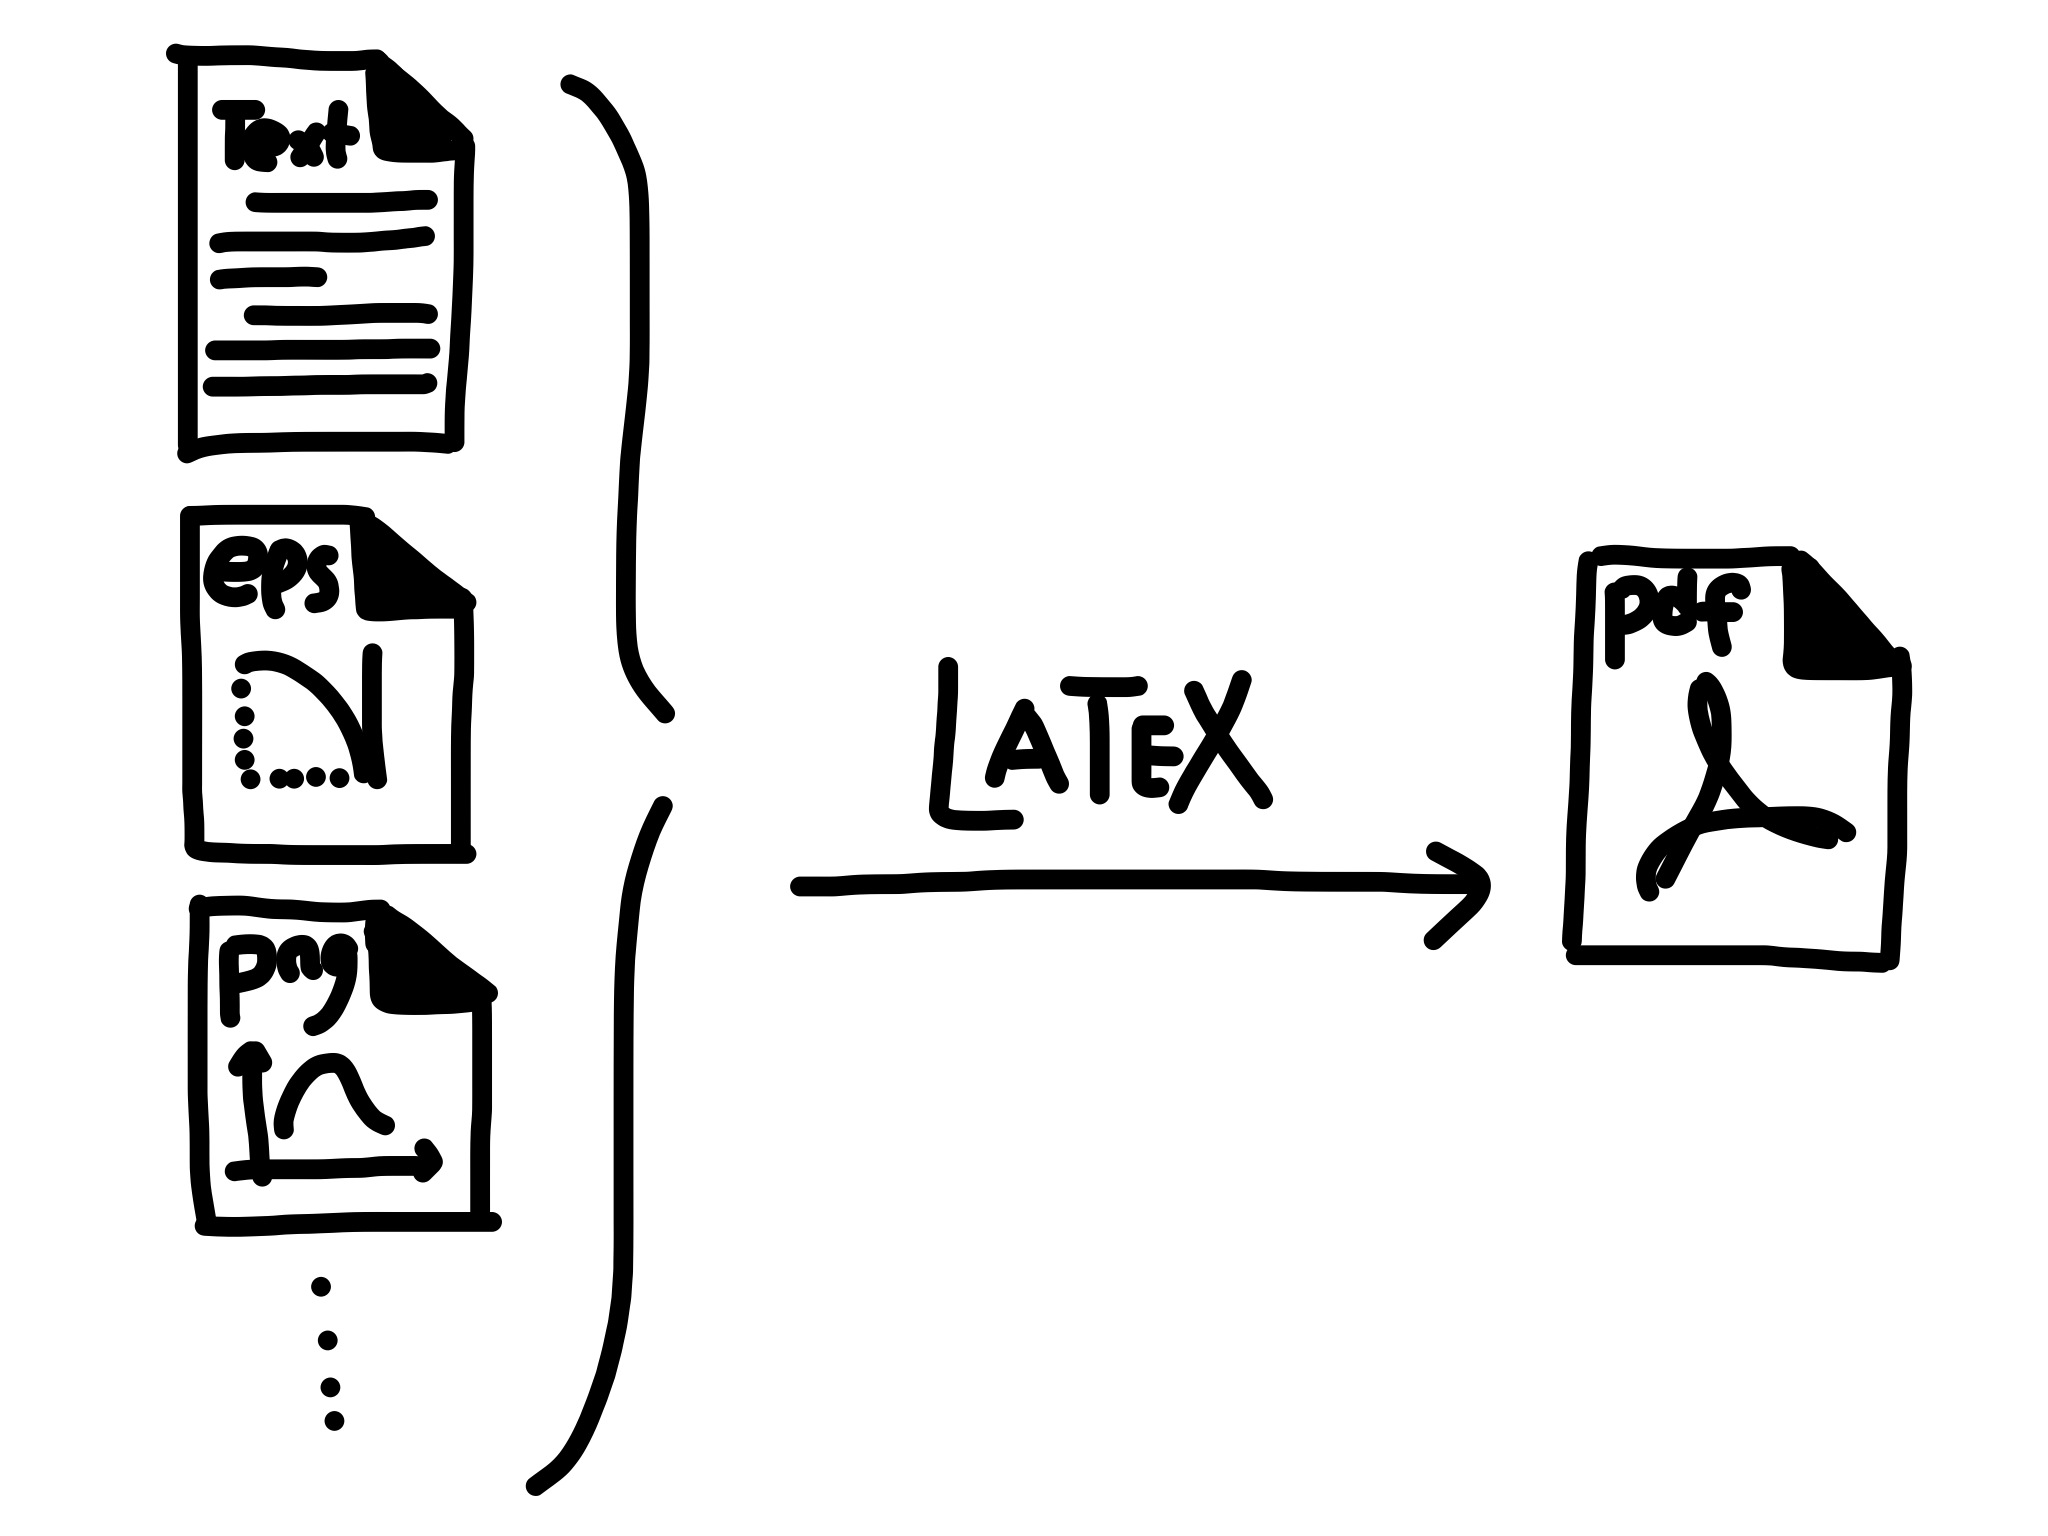
\includegraphics[width=6cm]{latex_zj.jpg} 
\caption{\label{latex}\LaTeX 工作方式}
\end{figure}

公司选用\LaTeX 并采用统一的模板,好处为:
\begin{enumerate}
\item 统一公司文档的风格。
\item 方便不同的人在不同平台下编辑和修改同一个文档。
\item 相比其他排版软件,\LaTeX 崩溃的概率小;文本文档损坏的概率也小。
\item \LaTeX 排出的版面更漂亮
\item \LaTeX 免费。
\end{enumerate}
坏处是用户编辑\TeX 文本文档时不够直观。对此公司的建议顺序是:
\begin{enumerate}
\item 使用纯文本编辑器编辑\TeX 文档,找一个\LaTeX 手册放在手边。(跟 Linux 一样,\LaTeX 常用的语法也就那么几页纸的事\cite{oetiker1995not}。)
\item 用 lyx 编辑。
\item 其他可输出\TeX 文档的软件。要求生成的\TeX 文档适于人工阅读。
\end{enumerate}

\section{软件和模板使用方法}
目前我们公司使用的\LaTeX 发行包为 texlive,你可以直接使用公司 helium 服务器上的,也可以在自己的电脑上安装一份来用。以下分别介绍。

\subsection{在服务器上使用\LaTeX}

模板及示例文件在服务器的\filename{/home/public/document/template}路径下。

首先,我们需要设置使用TexLive软件所需的环境。
\begin{lstlisting}[language=sh,caption={直接使用 Helium 上的 \LaTeX}]
# Set the path environment of texlive 
  source /usr/local/texlive/setenv.sh
# Or to make it permanent, you can do:
#    cat /usr/local/texlive/setenv.sh >> $HOME/.bash_profile
\end{lstlisting}

其次,每个用户需要将最新的模板文件安装到\filename{\$HOME/texmf/tex/latex/cgdrep}目录下,
其步骤如下:
\begin{lstlisting}[language=sh,caption={安装\LaTeX{}模板}]
# Unpack the template
  tar xf /home/public/document/template/cgdrep.tar.gz
  cd cgdrep
# Install the template files
  ./install.sh
\end{lstlisting}

现在,我们可以使用 \LaTeX 模板的示例了:
\begin{lstlisting}[language=sh,caption={直接使用 Helium 上的 \LaTeX}]
# test the LaTeX example
  cd example/latex
  make
# There should be several new files and one of them is main.pdf
  evince main.pdf &
\end{lstlisting}

\subsection{在自己电脑上安装 texlive}
目前我们使用的 texlive 是个未经简化的庞大的包,iso 镜像文件 2.4G,安装后需要 3.5G 的硬盘空间。
镜像文件下载路径为:\filename{/home/public/software/tex/texlive2013}。
对于 Linux 系统,可能需要几个字体文件,文件在 \filename{/home/public/sofware/tex/texlive2013/win\_fonts.tar.gz}。

假设你准备把字体安装在 /usr/share/fonts/TTF/。安装为:
\begin{lstlisting}[language=sh,caption={安装字体}]
# copy the font files
  tar -xzvf win_fonts.tar.gz && sudo cp -r win_fonts /usr/share/fonts/TTF/
# active the fonts
  sudo fc-chache -fv
\end{lstlisting}

假设你准备把 texlive 安装在 \filename{/usr/local/tex} 。方法为:
\begin{lstlisting}[language=sh,caption={安装 Texlive}]
# mount the iso file
  sudo mount -o loop texlive2013-20130530.iso /mnt/dvd  && cd /mnt/dvd
# install it
  export TEXLIVE_INSTALL_PREFIX=/usr/local/tex
  perl install-tl
# then follow the instructions to set the path environment
  export PATH=/usr/local/texlive/2013/bin/x86_64-linux:$PATH
\end{lstlisting}

对于 Windows 用户,原镜像文件也支持 Windows。请阅读镜像文件里的说明文件。

\section{关于 lyx}
lyx 是一个直观的编辑\TeX 文件的编辑器。

不需要 lyx 的人可以跳过这用节\footnote{脚注示例。}。


